\documentclass[../SimBALink.tex]{subfiles}
\begin{document}

\section{Motor model performance}
	xxx
	\subsection{Calibration}
		dafsd
		
		\subsubsection{Efficiency model}
			The motor efficiency model was derived from an efficiency plot provided by the manufacturer. 
			
			\begin{figure}[h]
				\centering
				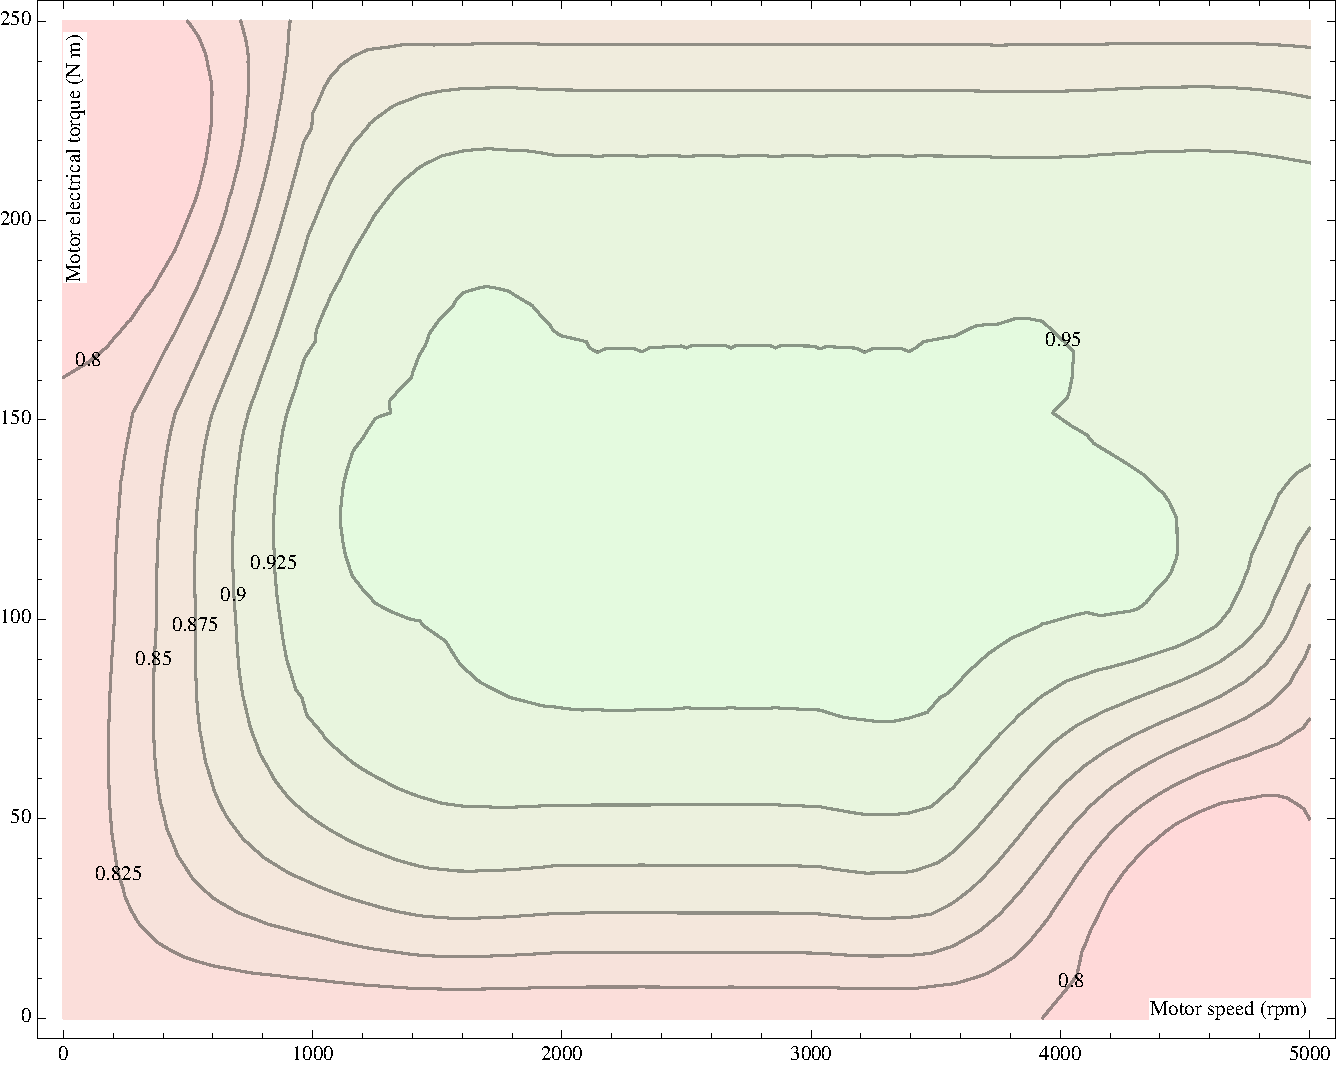
\includegraphics[width=4in]{../Model/Powertrain/Motor/Documentation/Figures/EMRAX_228HV_efficiency}
				\caption{Enstroj EMRAX 228HV - motor efficiency over operating range.}
			\end{figure}
			\FloatBarrier
			
			The efficiency plot is based on variables which are convenient to measure using an engine dynamometer and a power inverter. In future testing, the efficiency function will be derived from steady-state experimental data.
			
		\subsubsection{Equivalent-circuit parameters}
			The motor manufacturer specifies values for $L_d$, $L_q$, and $R$. Since the model performance was good without additional calibration of these values, they were used unchanged.
			
			The only equivalent-circuit parameter that was calibrated in the model was $\phi$, the permanent-magnet flux linkage.
						
			\begin{table}
				\centering
				\caption{Calibrated parameters in motor model}
				\label{table:motor_calibrated_parameters}
				\begin{tabular}{c | l | c | c}
					Symbol		&	Parameter			&	Initial guess value	&	Calibrated value	\\
					\hline
					$\phi$		&	Motor flux linkage		&	1 V rad/sec	 	&	-1.051 V rad/sec
				\end{tabular}
			\end{table}
			
			Since there was no calibration data available that included a motor torque output, the model was calibrated against a subset of the experimental data from RW-2x coastdown testing (the same dataset used for validating the overall vehicle model). The coastdown test data was chosen because it covered a wide range of vehicle speeds and motor currents.
			
			\begin{figure}[h]
				\centering
				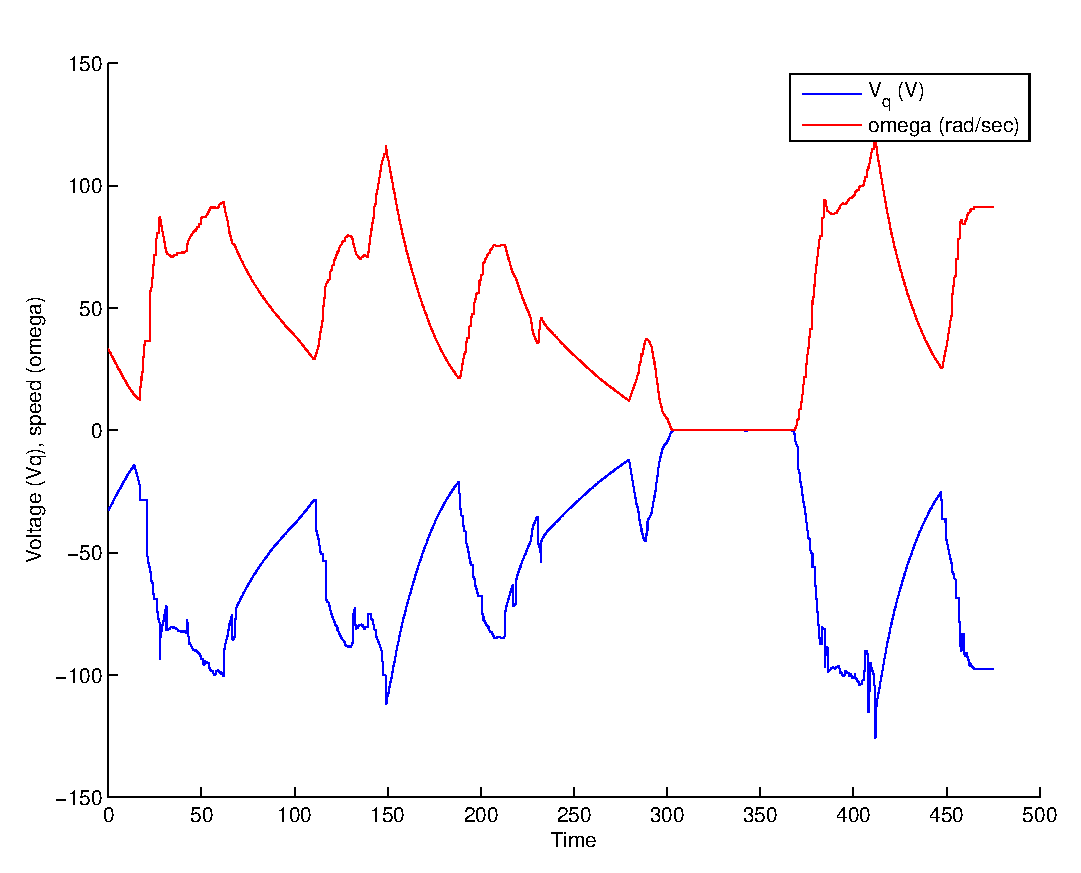
\includegraphics[width=5in]{../Model/Powertrain/Motor/Validation/EMRAX_228HV/Figures/228HV_coastdown_calibration_data}
				\caption{Coastdown dataset used for $\phi$ calibration.}
			\end{figure}
			\FloatBarrier
			
	\subsection{Model validation and quality of fit}
		The model was validated using the full coastdown dataset from RW-2x vehicle testing. Motor output torque was not directly measured during this testing, so the validation focused on accurate prediction of the motor equivalent-circuit voltages $V_d$ and $V_q$. 
		
		\begin{figure}[h]
			\centering
			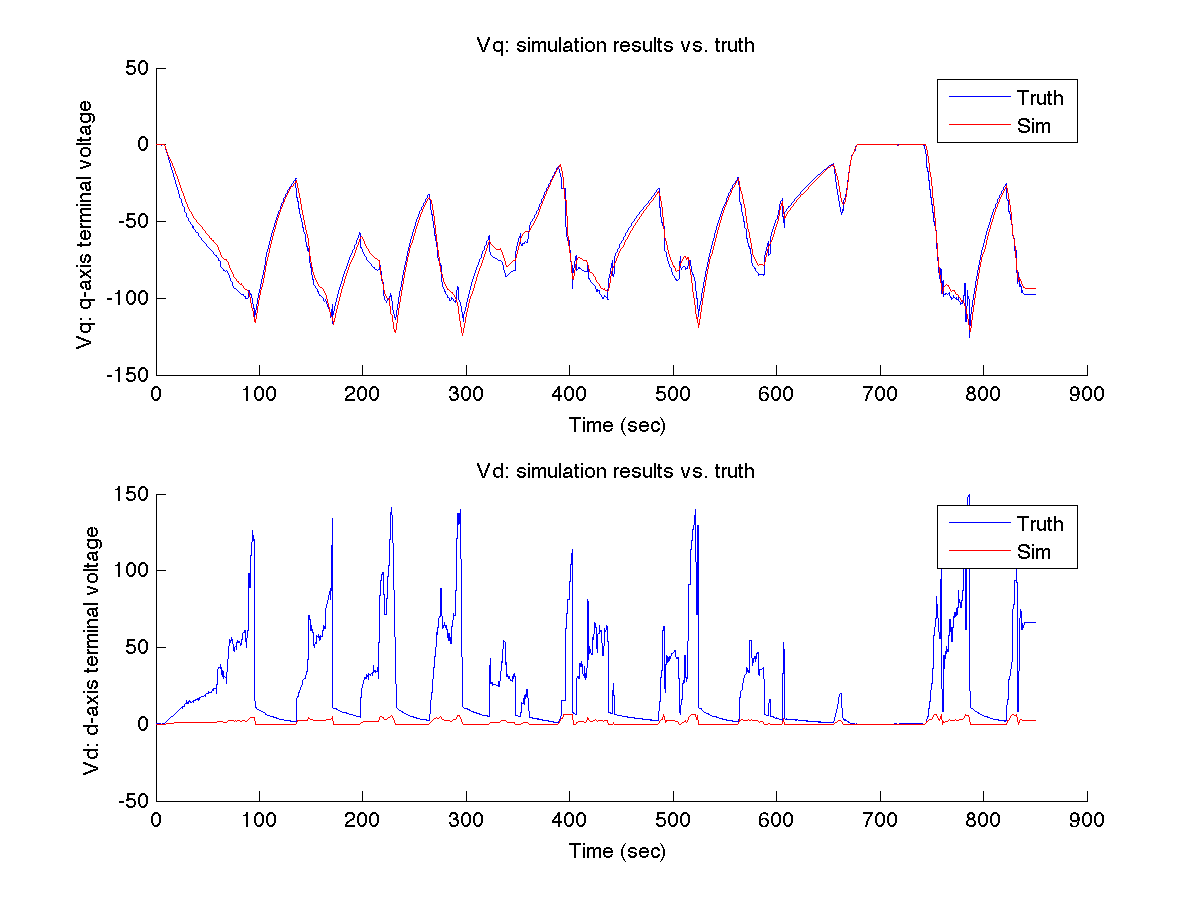
\includegraphics[width=\linewidth]{../Model/Powertrain/Motor/Validation/EMRAX_228HV/Figures/Vq_Vd}
			\caption{Motor model performance: simulated $V_q$, $V_d$ vs. measured data.}
		\end{figure}
		\FloatBarrier
		
		The model performance for $V_q$ is very good, even during transients. 
		
		The model does not predict $V_d$ well. Some possible sources of this error include:
		
		\begin{itemize}
			\item		Large applied voltages by the motor controller in an attempt to control for $I_d = 0$
			\item		Larger than expected coupling between the d- and q-axis circuits
			\item		Larger than expected $\frac{d i_d}{d t}$ or $L_d$
		\end{itemize}
		
		
\end{document}